\section{Convolution performance}
    We implemented two versions of the convolution algorithm as described before, the naïve version and the FFT version. We compared their performance when performing convolution on two $\Delta$Qs of equal bins.
    \begin{figure}[H]
        \begin{center}
            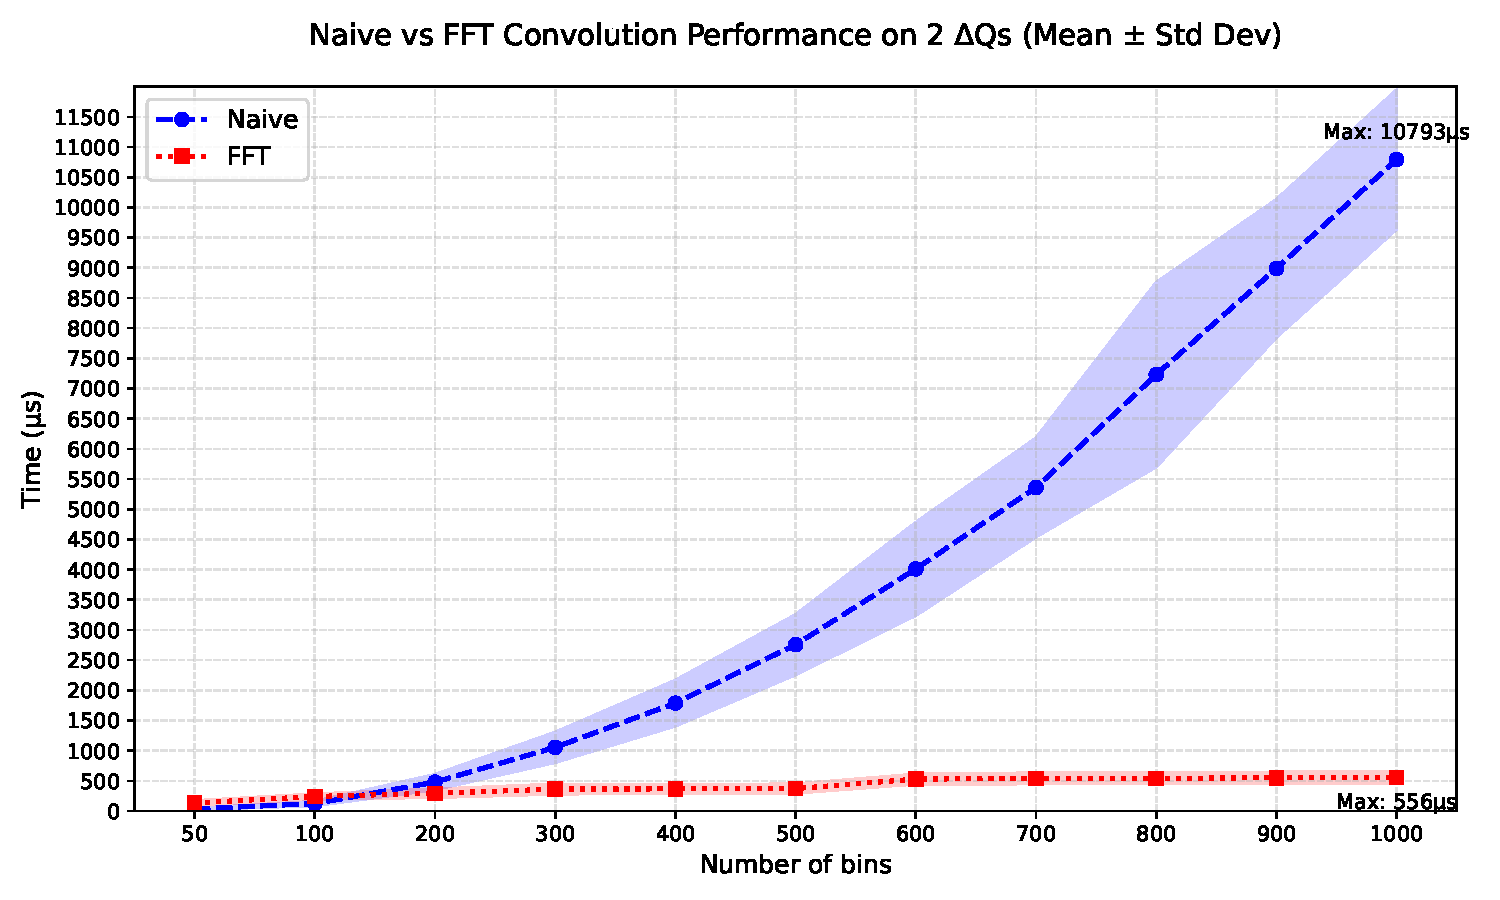
\includegraphics[width=0.85\textwidth]{img/conv_perf.pdf}
        \end{center}
        \caption{Performance comparison of two convolution algorithms}\label{fig:conv_perf}
    \end{figure}

    As expected, the naïve version has a time complexity of $\mathcal{O}(n^2)$ and quickly scales with the number of bins, this is clearly inefficient, as a more precise $\Delta$Q will result in a much slower program.

As for the FFT algorithm, it is slightly slower when the number of bins is lower than 100. This is due to the FFTW3 routine having slightly higher overhead.
